\section{Sprint 5}
\subsection{Sprint summary}
After sprint 4, the application had started to take form. Sprint 5 consisted of further development from prototype to something stable and functional, combined with a lot of important design choices. The customer expressed that he wanted to become even more involved with the development process by taking part in the sprint start meetings where tasks were estimated, prioritized and allocated resources. The customer also gave a lot of constructive feedback that lead to many major redesigns, particularly in the menus. We were made aware of that navigation in what was the main menu at the time could be a challenge. The team laid out user stories according to the system specification, and after discussing each point, the team and customer agreed to sprint layouts for the remainder of the project.
	
\subsection{Sprint burndown}



\begin{figure}[H]
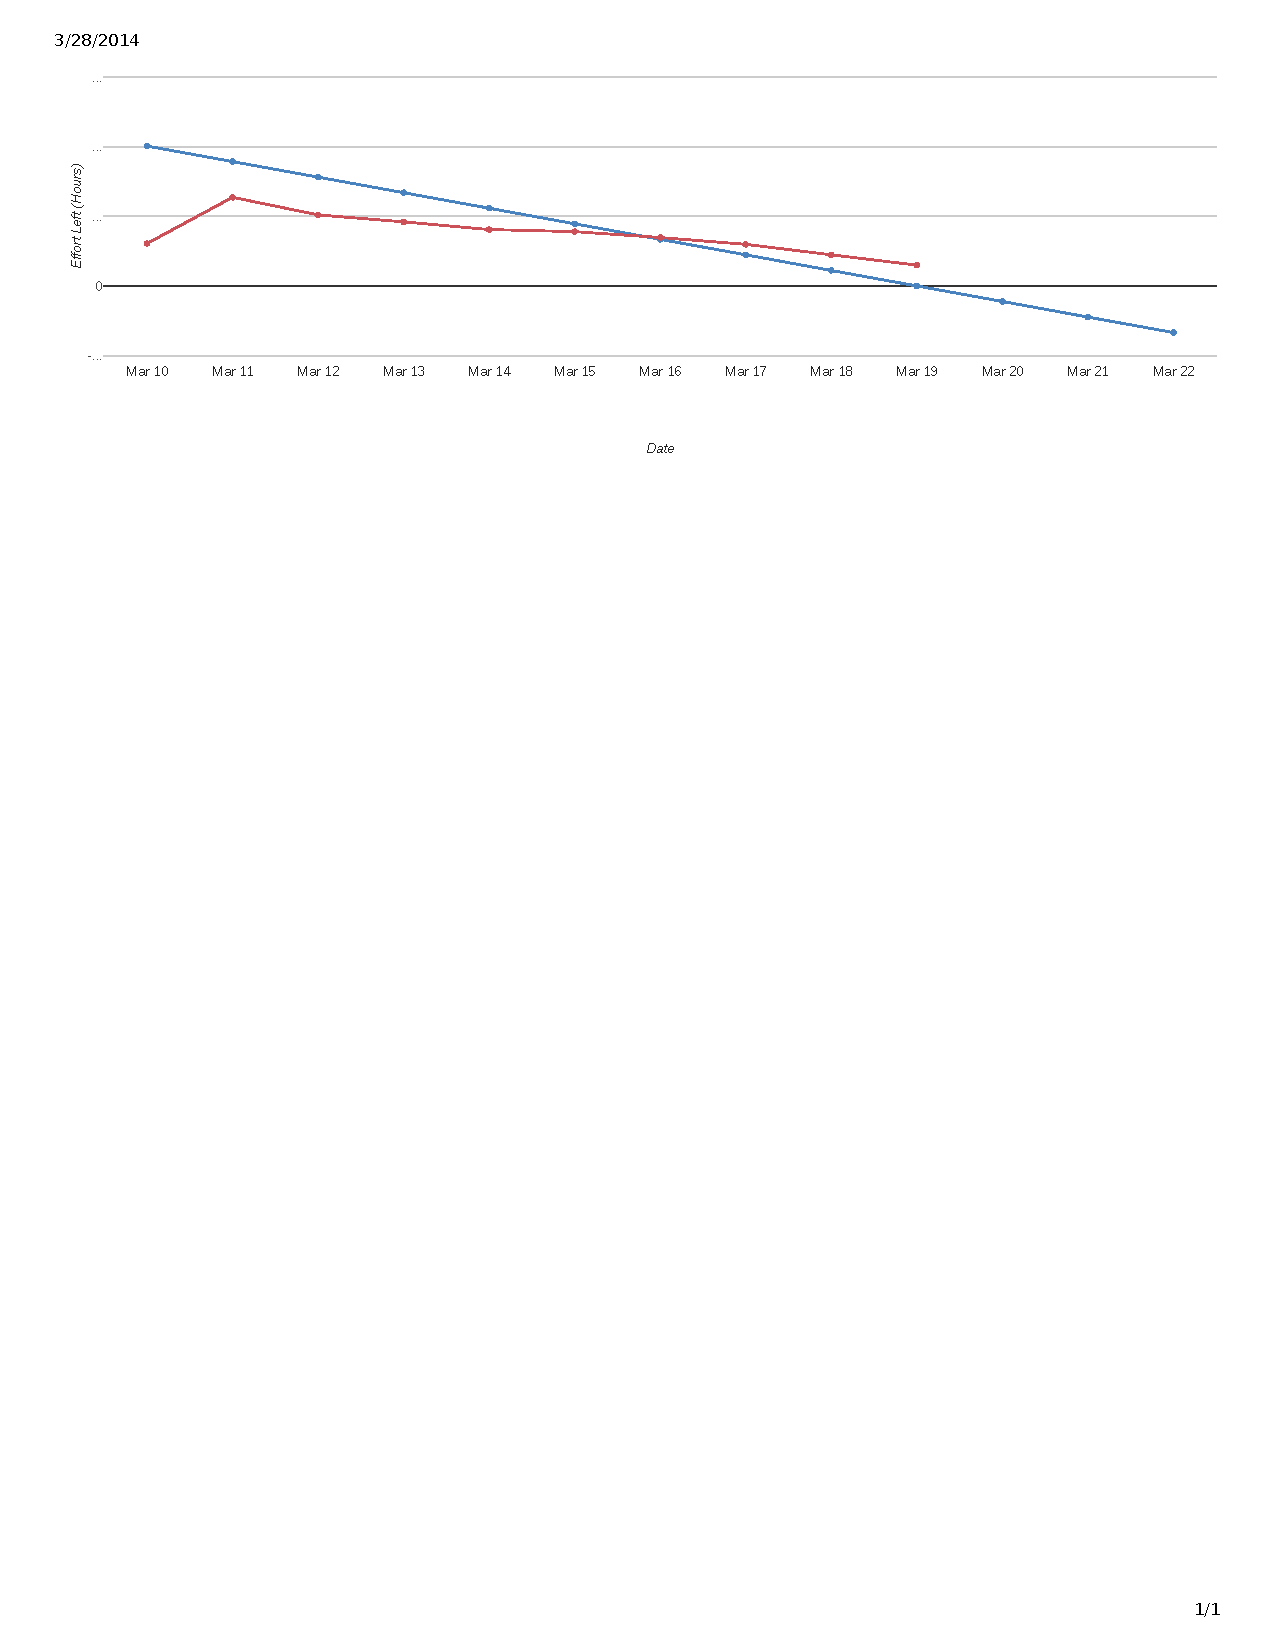
\includegraphics[width=\textwidth, trim= 1cm 21cm 1cm 1cm, clip=true]{ch/projectManagement/fig/burndown4.pdf}
\caption{Sprint 5 burndown chart}
\label{fig:sprint5burndown}
\end{figure}

\subsection{Sprint backlog}



\begin{table}[H]
	\begin{tabular}{|l|p{7cm}|p{2.2cm}|p{1.5cm}|p{1.5cm}|}%
		\hline \bfseries User story & \bfseries Details & \bfseries Hours\newline estimated & \bfseries Hours spent & \bfseries Hours left
		\csvreader[head to column names]{ch/projectManagement/sec/sprints/sprint5/userstories.csv}{}% use head of csv as column names
		{\\\hline \id & \title & \estimated & \spent & \left} \\\hline% specify your coloumns here
	\end{tabular}
    \caption{Sprint 3 backlog}
\end{table}

\subsection{Issues and solutions}
\label{sec:unbalancedWorkload}
During this sprint, the team evaluated whether the use of the team's available resources actually were fully exploited. It was acknowledged that our current Scrum master, Per Øyvind, had the best control of the development environment, which in turn lead to that the workload he got due to his position as Scrum master and his level of expertise, was too great. The team therefore decided that Lars Erik, which previously was our deputy project leader, was the best fit to be the new Scrum master.

It was also discussed whether the position ''Project leader'' actually was necessary, as it conflicted with one of the principles in Scrum. The team decided that we in fact thought the position was necessary, as the project leader and Scrum master simply distributed the Scrum master's traditional tasks between them. The main difference would be that the project leader would handle the administrative tasks, such as room booking for meetings and work sessions, and handle customer relations, while the Scrum master would handle the project administrative tasks, such as moderating the Scrum meetings, adding tasks to the backlog and Yodiz, and generate burndown charts.

\subsection{Work completed}
As mentioned above, the entire main menu was restructured. Where there had previously just been a list of tabs, these options were now divided by categories built on concepts. Naming the different functionalities under abstract concepts allows for much easier user navigation. The layout of many tabs were also revised upon request from the customer. Even thought the version the customer tested in sprint 4 was just a prototype, the feedback gave valuable insight to his vision for the application. 	Large amounts of work was done server side to allow storage and retrieval of data about consumption and registered devices. 

\subsection{Sprint review}
The sprint had some goals that were not met. Data synchronization was not implemented and all dummy data was not yet replaced by data from the server based on user credentials.